\chapter{Introdução}

\section{Contextualização e Justificativa}

O entretenimento digital vem sendo cada vez mais popular entre as crianças e os adolescentes e atualmente é tão abrangente que engloba um público mais adulto e maduro
e um outro grupo de jogadores casuais que antigamente não jogavam por geralmente encontrar dificuldades em manipular o joystick usual,que agora jogam videogames como
o Nintendo Wii, ou usando acessórios como o PS Move no Playstation 3 e o Kinect no Xbox360. Muitos fabricantes de jogos eletrônicos, se empenham em criar efeitos mais atrativos para os
usuários, uns recorrem a gráficos e animações mais realistas enquanto outros se preocupam em criar  uma experiência de jogabilidade inovadora.\cite{WiiWillRockYou}

\begin{figure}[h]
    \center
    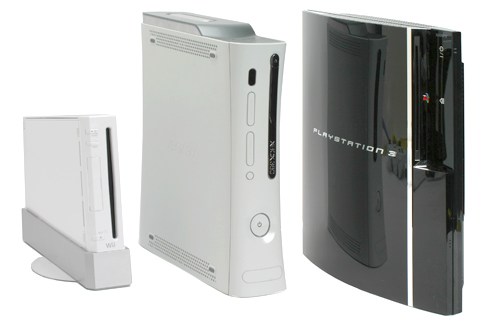
\includegraphics[scale=0.40]{imagens/os3consoles.jpg}
    \label{os3consoles}
    \caption{Nintendo Wii, Xbox 360 e PS3}
\end{figure}

Nos jogos fisicamente interativos\footnote{\textit{What is motion-controlled gaming? Definition from WhatIs.com.}
http://whatis.techtarget.com/definition/motion-gaming.html. Acesso  em: 14/09/2011.}, o usuário movimenta partes do corpo para atuar direta ou indiretamente com
o jogo. Esses movimentos são geralmente capturados por controles com sensores de movimento na maioria das vezes com uma câmera, que através de processamento de
imagens, serão traduzidos e retornados como comandos no ambiente virtual do jogo. Essa interação pode ser através de um objeto animado que representa o jogador,
chamado de avatar realizando ações que o usuário realiza na área de visão da câmera.

Atualmente a indústria de jogos tem um movimento financeiro comparável a indústria cinematográfica e um retorno lucrativo muitas vezes maior.
Ela cresceu muito e enquanto antigamente era comum apenas um programador desenvolver um jogo, hoje é necessário quase sempre, centenas de pessoas e milhares de
dólares e alguns anos para a conclusão de um projeto. No fim do ano passado \textit{Call of Duty: Black Ops}\footnote{\textit{Call of Duty: Black Ops} é um jogo de
tiro em primeira pessoa desenvolvido pela Treyarch, editado pela Activision e lançado mundialmente em 9 de novembro de 2010 para as plataformas Microsoft Windows,
 Xbox 360, Playstation 3, Wii e Nintendo DS.} foi o maior lançamento da história do entretenimento,
vendendo no dia do lançamento 5,6 milhões de cópias nos Estados Unidos e Reino Unido, já vendeu mais de 13 milhões e é o título mais vendido da história no mercado
americano. Apenas para efeito de comparação, o filme \textit{Avatar}\footnote{\textit{Avatar} é um filme americano de ficção científica de 2009, escrito e dirigido
por James Cameron, que está em primeiro lugar no ranking de bilheteria, que rendeu US\$ 2,78 bilhões.} vendeu 3,2 milhões de DVDs e Blu-Rays mundialmente no dia do
 lançamento.\cite{TamanhoIndustriaGames}

Entretenimento por computador ou videogames fazem um papel importante na vida de muitas pessoas e os pais acreditam que existe um impacto positivo em jogar por videogames.
De acordo com a Associação de Software de Entretenimentos do Estados Unidos\cite{ESA}, 72\% dos chefes de família jogam por computador ou vídeo games,
91\% das vezes os país estão presentes na hora que um jogo é alugado ou comprado. 68\% dos pais acreditam que jogos fornecem estimulação mental ou educacional,
57\% acreditam que os jogos auxiliam a família a passar mais tempo junta e 54\% acreditam que ajudam as crianças a se juntarem com amigos. 59\% acreditam que esses
jogos proporcionam mais atividade física hoje do que 5 anos atrás.45\% dos pais jogam com seus filhos no mínimo semanalmente, um aumento de 36\% em 2007.
A idade média do jogador é 37 anos, 82\% tem idade acima de 18 anos, 29\% dos jogadores tem idade acima de 50 anos, um aumento de 9\% em relação a 1999.
Um cenário que é certo de aumentar nos próximos anos com lares e centros de idosos em todo o país incorporando vídeo game em suas atividades.
65\% jogam com outros jogadores pessoalmente. 33\% deles disseram que jogar por computador ou vídeo game é a atividade de entretenimento favorita deles.
Os jogadores adultos já jogam a uma média de 12 anos. Os consumidores gastaram um total de mais de 25 bilhões com a indústria de jogos em 2010.
Todo esse cenário nos revela como existe a pratica regular de se jogar tanto por crianças quanto por adultos, assim como o retorno financeiro envolvido nessa
indústria. É importante então observar e se estudar os efeitos dessa rotina.

Esse trabalho apresenta uma introdução aos fundamentos teóricos do curso de graduação ciência da computação aplicados ao desenvolvimento de jogos eletrônicos
fisicamente interativos.Ao final, há o detalhamento do processo de desenvolvimento de um jogo demonstrativo, que acompanha a monografia.

\section{Grandes empresas e jogos fisicamente interativos}

Quando o Nintendo Wii começou a usar controles(figura \ref{wiimote}) simples de se usar com sensores de movimentos e com preço mais acessível, criando um ramo de jogos onde sensação
de imersão se dava pelos movimentos físicos que o jogador fazia ao invés de gráficos superiores, fez um grande sucesso, atraiu um grupo de consumidores diferente
e conseguiu competir em vendas contra os consoles  da concorrência que possuem hardware superior, porem alguns anos depois a Microsoft e Sony observando o sucesso
do estilo de jogo, construíram acessórios para desenvolverem também seu jogos fisicamente interativos.

\begin{figure}[h]
    \center
    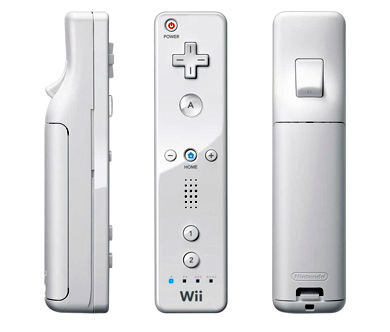
\includegraphics[scale=0.45]{imagens/wiimote.jpg}

    \caption{Controle Wiimote da Nintendo Wii}
    \label{wiimote}
\end{figure}

A Sony desenvolveu um controle similar ao da Nintendo, chamado PS Move(figura \ref{psmove}), o aparelho possui sensores com desempenho melhores, funciona junto com uma webcam,
chamada de que PSeye(figura \ref{pseye}), que
possui uma taxa de captura de quadros acima da média, o controle possui uma esfera na extremidade superior que acende com uma luz que varia de cor, essa luz
permite que a webcam identifique o controle mesmo em ambientes completamente escuros, o fato de ter uma webcam trabalhando em conjunto com os controles, melhora
a imersão e faz com que seja mais difícil o usuário "enganar" o jogo, como acontecia por exemplo no Nintendo Wii, era possível jogar um jogo de luta e executar
os socos simplesmente balançando os controles, a PSeye, no caso da Sony, identifica quando o controle esta mais perto ou mais distante da webcam, colocada em
cima da televisão, balançar os sensores do controle nessa situação não levará o avatar a socar, como acontecia no Wii, pois a câmera não estará capturando a
aproximação dos controles em relação a ela.\cite{MotionGamingReview}

A Microsoft criou um acessório diferenciado, chamado Kinect(figura \ref{kinect}), com preço bem acima dos concorrentes, eliminou a necessidade de qualquer controle para jogar, o hardware desse
acessório contém 2 câmeras, 4 microfones, acelerômetro, ventoinha, projetor infra-vermelho e diversos chips para que o processamento fosse feito o mínimo no
console.\cite{InsideKinect}

Apesar da Microsoft fornecer os drivers para que o acessório possa ser reconhecido pelo sistema operacional Windows e mais recentemente o GNU/Linux, o preço está
em torno de R\$ 400,00, o que a torna um acessório inviável para muitos usuários de computador,  contra, por exemplo R\$ 80,00 da PSeye,
preço melhor quando comparada a outras webcams da mesma categoria.

\begin{figure}[h]
    \center
    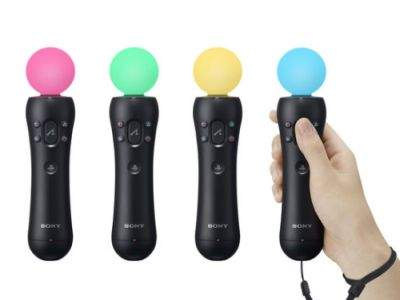
\includegraphics[scale=0.45]{imagens/psmove.jpg}

    \caption{Controle PSmove do PS3}
    \label{psmove}
\end{figure}

\begin{figure}[h]
    \center
    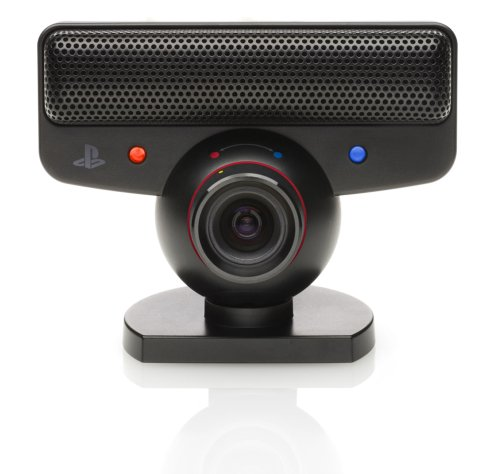
\includegraphics[scale=0.25]{imagens/pseye.jpg}

    \caption{Camera  PSeye do PS3}
    \label{pseye}
\end{figure}

\begin{figure}[h]
    \center
    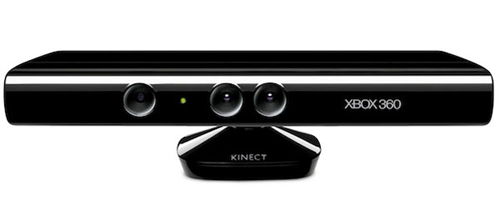
\includegraphics[scale=0.35]{imagens/kinect.jpg}

    \caption{O Kinect da Microsoft}
    \label{kinect}
\end{figure}

\section{Definindo o Problema}

Esse projeto não utilizará nenhum equipamento específico, diferente da maioria
dos trabalhos relacionados citados no segundo capítulo, será desenvolvido para câmeras
web doméstica em microcomputadores.

O projeto tem como desafio criar um rastreio do corpo  do usuário, ou alguma parte dele
ou algum objeto que o mesmo esteja segurando.Será preciso calcular a posição do usuário
em relação a câmera e para que essa experiência seja em fluente do
ponto de vista de taxa de atualização entre os movimentos que são executados e o retorno
por parte do ambiente gráfico, será importante uma boa taxa de quadros assim como
uma taxa aceitável de detecção para cada uma deles.A maioria dos algoritmos de
detecção consomem muito processamento. Essa detecções precisarão ser feitas
rapidamente, para que o programa consiga rodar em tempo real. Com uma baixa
taxa de frames por segundo, o usuário terá um atraso entre o movimento que ele executou
e a resposta do programa.

Os protótipos estão sendo desenvolvidos utilizando a linguagem Python, com o
auxílio da biblioteca OpenCV, para processamento de imagem. Para a modelagem
do ambiente virtual, foi utilizado a biblioteca OpenGL, mas ainda está sendo
estudada a possibilidade de se utilizar a biblioteca Pygame ou o programa Blender.
O sistema pode ser visualizado na figura \ref{Diagrama}.

\begin{figure}[h]
    \center
    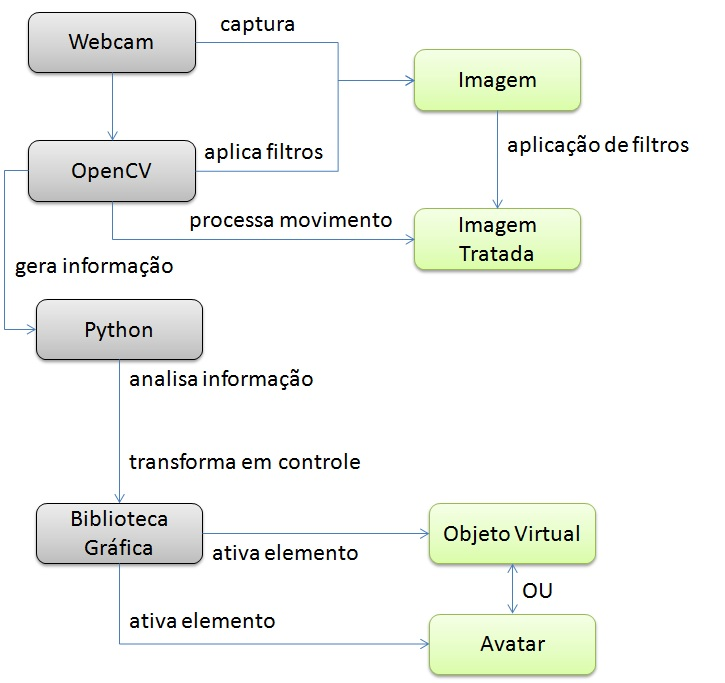
\includegraphics[scale=0.50]{imagens/Diagrama.jpg}

    \caption{Diagrama de blocos do projeto}
    \label{Diagrama}
\end{figure}

\section{Objetivos do Projeto}

Desenvolver alguma técnica para capturar os movimentos do usuário através de uma webcam que depois de processado e interpretado irá ser associado a um elemento
que o representará no ambiente virtual.

\subsection{Objetivo geral}

Estabelecer um esquema modular e criar uma ferramenta para incentivar o desenvolvimento e pesquisas de tecnologias de software para jogos fisicamente interativos
baseados em princípios de imersão.

\subsection{Objetivo específico}

Implementar um ou mais exemplos de mini-jogos fisicamente interativos, investigando os requisitos mínimos de hardware necessários, como a taxa mínima de quadros
capturados pela webcam, \textit{clock} do processador e memória RAM.

\section {Apresentação da monografia}

No capítulo 2, são apresentados os trabalhos relacionados, técnicas e algoritmos para rastreamento de movimentos,
objetos, captura e aplicação em ambientes virtuais ou jogos.
O terceiro capítulo é dedicado à fundamentação teórica necessária para o entendimento
desse trabalho.Explica, entre outros, os princípios de processamento de imagens
envolvidos na detecção e reconhecimento de pessoas ou objetos e seus respectivos movimentos,
assim como os princípios de computação gráfica envolvidos no ambientes virtuais,
avatares e suas animações.
O capítulo 4 é focado no desenvolvimento do trabalho, explicando todas as etapas de
implementação do projeto e seus resultados.
Finalmente o quinto capítulo apresenta as conclusões e considerações finais do projeto e sugestões
para trabalhos futuros.

